\documentclass[12pt]{article}
\usepackage{amsmath,amssymb,amsthm}
\usepackage{graphicx}
\usepackage{microtype}
\usepackage{etoolbox}
\usepackage[colorlinks=true,linkcolor=blue,citecolor=blue,urlcolor=blue]{hyperref}
\usepackage[margin=1in]{geometry}
\makeatletter
\let\inputresultrows\@@input
\setlength{\@fptop}{0pt}
\setlength{\@fpsep}{12pt plus 2pt minus 2pt}
\makeatother
\renewcommand{\topfraction}{0.9}
\renewcommand{\bottomfraction}{0.8}
\renewcommand{\textfraction}{0.07}
\renewcommand{\floatpagefraction}{0.85}
\setcounter{topnumber}{3}
\setcounter{totalnumber}{4}
\setlength{\textfloatsep}{10pt plus 2pt minus 2pt}
\setlength{\intextsep}{10pt plus 2pt minus 2pt}
\setlength{\floatsep}{8pt plus 2pt minus 2pt}
\apptocmd{\thebibliography}{\setlength{\itemsep}{0pt}\setlength{\parsep}{0pt}}{}{%
  \PackageError{revision-layout}{Bibliography spacing patch failed}{Check the document class.}}

\title{Supplementary Appendix for\\
Randomized Kolmogorov--Smirnov Calibration\\
for Fitted Discrete Single-Cell Residual Diagnostics}
\author{Elvis Han Cui\thanks{Corresponding author: elviscuihan@g.ucla.edu}\\
College of Environmental and Resource Sciences, Zhejiang University;\\
Department of Biostatistics, University of California, Los Angeles\\[0.6em]
Yihao Li\\
College of Environmental and Resource Sciences, Zhejiang University; Genentech\\[0.6em]
Zhuang Liu\\
College of Environmental and Resource Sciences, Zhejiang University; Google}
\date{Statistics in Biosciences}

\newtheorem{theorem}{Theorem}
\newtheorem{proposition}[theorem]{Proposition}
\newtheorem{corollary}[theorem]{Corollary}
\newtheorem{definition}[theorem]{Definition}
\newtheorem*{fact}{Fact}
\theoremstyle{remark}
\newtheorem{remark}[theorem]{Remark}

\newcommand{\Prob}{\mathbb{P}}

\begin{document}
\begin{center}
{\LARGE\bfseries Supplementary Appendix for\par}
\vspace{0.5em}
{\Large\bfseries Randomized Kolmogorov--Smirnov Calibration\par}
{\Large\bfseries for Fitted Discrete Single-Cell Residual Diagnostics\par}
\vspace{1.0em}
{\large Elvis Han Cui\textsuperscript{*}, Yihao Li, and Zhuang Liu\par}
\vspace{0.4em}
{\small College of Environmental and Resource Sciences, Zhejiang University\par}
{\small Department of Biostatistics, University of California, Los Angeles\par}
{\small Genentech; Google\par}
\vspace{0.4em}
{\small \textsuperscript{*}Corresponding author: elviscuihan@g.ucla.edu\par}
\vspace{0.4em}
{\small Statistics in Biosciences\par}
\end{center}
\vspace{1em}

\section*{A. One-Sample Crossing Formula}

This appendix expands the volume calculation used in the proof of the
Smirnov-Birnbaum-Tingey one-sided crossing formula. Work on the uniform scale.
Let $U_{(1)}<\cdots<U_{(n)}$ be the order statistics of independent
$\operatorname{Unif}(0,1)$ variables and set $U_{(0)}=0$, $U_{(n+1)}=1$.
On $[U_{(j)},U_{(j+1)})$, the empirical distribution function equals $j/n$.
Thus the first lower crossing at $t_j=\epsilon+j/n$ occurs when
\[
U_{(i)}\le \epsilon+\frac{i-1}{n},\quad i=1,\ldots,j,
\qquad
U_{(j+1)}>\epsilon+\frac{j}{n}.
\]
For $j=0$, this gives
\[
\mathbb{P}\{\tau_n(\lambda)=\epsilon\}=(1-\epsilon)^n.
\]
For $j\ge1$, the desired probability is $n!V_j$, where
\begin{align*}
  V_j
  &=\int_0^\epsilon\int_{u_1}^{\epsilon+\frac{1}{n}}\cdots
    \int_{u_{j-1}}^{\epsilon+\frac{j-1}{n}}
    \int_{\epsilon+\frac{j}{n}}^1\int_{u_{j+1}}^1\cdots
    \int_{u_{n-1}}^1 \\
  &\qquad du_n\cdots du_{j+2}\,du_{j+1}\,du_j\cdots du_2\,du_1 .
\end{align*}
Since $u_j\le\epsilon+(j-1)/n<\epsilon+j/n\le u_{j+1}$, this simplex
separates into the product
\begin{align*}
V_j
&=\left(\int_0^\epsilon\int_{u_1}^{\epsilon+\frac{1}{n}}\cdots
  \int_{u_{j-1}}^{\epsilon+\frac{j-1}{n}}
  du_j\cdots du_2\,du_1\right)\\
&\quad\times
\left(\int_{\epsilon+\frac{j}{n}}^1\int_{u_{j+1}}^1\cdots
  \int_{u_{n-1}}^1
  du_n\cdots du_{j+2}\,du_{j+1} \right).
\end{align*}
The second factor is the ordinary ordered-simplex volume
\[
\frac{(1-\epsilon-j/n)^{n-j}}{(n-j)!}.
\]
The first factor is the classical Birnbaum-Tingey simplex identity
\[
\int_0^\epsilon\int_{u_1}^{\epsilon+\frac{1}{n}}\cdots
    \int_{u_{j-1}}^{\epsilon+\frac{j-1}{n}}
    du_j\cdots du_2\,du_1
    =\epsilon\frac{(\epsilon+j/n)^{j-1}}{j!}.
\]
Therefore
\[
\mathbb{P}\left\{\tau_n(\lambda)=\epsilon+\frac{j}{n}\right\}
=n!V_j
=\epsilon\binom{n}{j}
\left(\epsilon+\frac{j}{n}\right)^{j-1}
\left(1-\epsilon-\frac{j}{n}\right)^{n-j}.
\]
Summing the mutually exclusive first-passage events gives
\[
\mathbb{P}(D_n^->\epsilon)
=(1-\epsilon)^n+\epsilon\sum_{j=1}^{\lfloor n(1-\epsilon)\rfloor}
\binom{n}{j}
\left(\epsilon+\frac{j}{n}\right)^{j-1}
\left(1-\epsilon-\frac{j}{n}\right)^{n-j}.
\]

\section*{B. Exact two-sample recursion}

Under $F=G$ and continuity, every pooled ordering of the $n$ observations from
the first sample and the $m$ observations from the second sample is equally
likely. At lattice point $(i,j)$ the one-sided empirical difference is
$i/n-j/m$. Counting paths that avoid the half-plane
$i/n-j/m\ge\delta$ gives the recursion in
Proposition~\ref{prop:one-wall-recursion}. The total number of
pooled orderings is $\binom{n+m}{n}$, so dividing the count of admissible paths
by this total gives the finite-sample probability exactly.



\section*{C. Fixed-null crossing formulas}

The following sections collect the finite-sample KS crossing derivations and
fixed-null limiting identities used as background for the fitted residual
diagnostics in the main text.

\section{One Sample: The First Crossing Time}\label{sec:one-sample-one-sided}

Let $X_1,\ldots,X_n$ be a random sample with continuous distribution function $F$ and let $F_n$ be its empirical counterpart:
\[
F_n(t)=\frac{1}{n}\sum_{i=1}^n\mathbb{I}(X_i\le t).
\]
Define the normalized empirical process by
\[
Z_n(t)=\sqrt{n}\left(F_n-F\right)(t)
\]
and let $D_n^{+}$ and $D_n^-$ denote the one-sided Kolmogorov-Smirnov statistics:
\[
D_n^+=\sup_{t}\frac{Z_n(t)}{\sqrt{n}}=\sup_t(F_n(t)-F(t)),
\]
\[
D_n^-=\sup_{t}\frac{-Z_n(t)}{\sqrt{n}}=\sup_t(F(t)-F_n(t)).
\]

Here the supremum becomes literal. Between observations the centered empirical
process drifts downward; at an observation it jumps upward. A lower-boundary
crossing therefore cannot occur everywhere on the line, but only at a small
set of lattice points. The next theorem is the classical exact answer, written
in this first-passage language.

\begin{figure}[t]
\centering
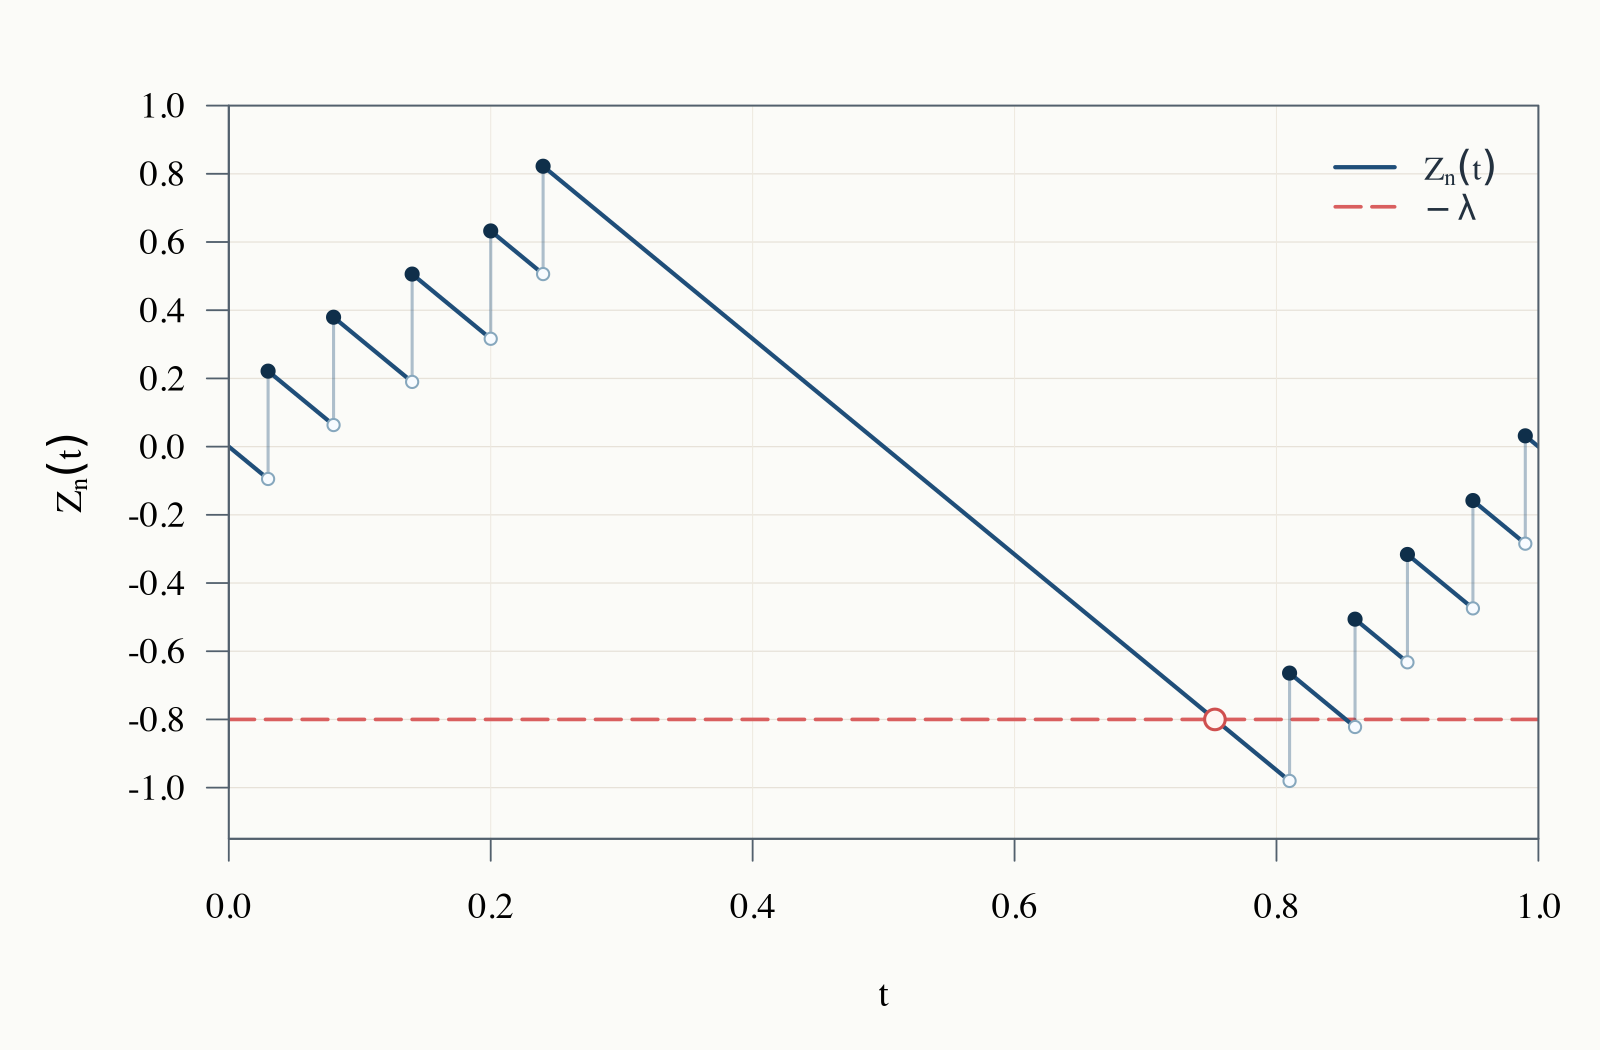
\includegraphics[width=0.82\textwidth]{figs/Zn.png}
\caption{A one-sample empirical process on the uniform scale for $n=10$. The
blue path is $Z_n(t)=\sqrt n\{F_n(t)-t\}$; it drifts downward between
observations and jumps upward at sample points. The red line is the lower
boundary $-\lambda$ with $\lambda=0.8$. The highlighted point is the first
boundary crossing, reducing the KS tail calculation to the finite hitting-time
question $t=\lambda/\sqrt n+j/n$.}
\label{fig:zn-crossing}
\end{figure}

\begin{theorem}[Smirnov-Birnbaum-Tingey \cite{birnbaum1951one}]
Let $0<\epsilon<1$ and set $\lambda=\sqrt{n}\epsilon$. Define
\[
\tau_n(\lambda)=\inf_t\{t:Z_n(t)\le-\lambda\}
\]
as the first time that $Z_n(t)$ hits $-\lambda$. Then
\begin{align}
    \mathbb{P}\left(D_n^->\epsilon\right)
    &=(1-\epsilon)^n+\epsilon\sum_{j=1}^{\lfloor n(1-\epsilon)\rfloor}\binom{n}{j}
    \left(\epsilon+\frac{j}{n}\right)^{j-1}
    \left(1-\epsilon-\frac{j}{n}\right)^{n-j}.
\end{align}
On the uniform scale, the corresponding first-passage probabilities are
\begin{align}
    \mathbb{P}\{\tau_n(\lambda)=\epsilon\}
    &=(1-\epsilon)^n,\\
    \mathbb{P}\left\{\tau_n(\lambda)=\epsilon+\frac{j}{n}\right\}
    &=\epsilon\binom{n}{j}\left(\epsilon+\frac{j}{n}\right)^{j-1}
    \left(1-\epsilon-\frac{j}{n}\right)^{n-j}
\end{align}
for $j=1,\ldots,\lfloor n(1-\epsilon)\rfloor$.
\end{theorem}

\begin{remark}
The reduction to $F(t)=t$ is distribution-free: after the probability integral transform, the distributions of $D_n^+$ and $D_n^-$ do not depend on $F$. On the original scale, the hitting locations are obtained by applying the generalized inverse $F^{-1}$ to the uniform-scale values $\epsilon+j/n$.
\end{remark}

\begin{remark}
The hitting time $\tau_n(\lambda)$ is discrete, although $\tau_n(\lambda)=+\infty$ may occur with positive probability. The process $Z_n(t)$ decreases between jump points; at each observation $X_i$, it jumps by $1/\sqrt{n}$. If $Z_n(t)$ does not cross below $-\lambda$ at $X_{(i)}$, the $i$-th order statistic, it must wait another $1/n$ in transformed time before crossing becomes possible. The first possible hitting time is $\epsilon=\lambda/\sqrt{n}$, corresponding to no observations below $\epsilon$. Thus the equation
\[
F_n(t)-t=-\epsilon
\]
has only finitely many possible solutions, all of the form $\epsilon+j/n$.
\end{remark}
\begin{proof}
It is enough to work on the uniform scale. Let
$U_{(1)}<\cdots<U_{(n)}$ be the order statistics of independent
$\operatorname{Unif}(0,1)$ variables, with $U_{(0)}=0$ and $U_{(n+1)}=1$.
On $[U_{(j)},U_{(j+1)})$, the empirical distribution function is $j/n$.
Thus the first crossing occurs at $t_j=\epsilon+j/n$ exactly when
\[
U_{(i)}\le \epsilon+\frac{i-1}{n}\quad(i=1,\ldots,j),
\qquad
U_{(j+1)}> \epsilon+\frac{j}{n}.
\]
The case $j=0$ gives $(1-\epsilon)^n$. For $j\ge1$, the probability is
$n!$ times the ordered-simplex volume cut out by these inequalities. The
Birnbaum-Tingey simplex identity \cite{birnbaum1951one} gives this volume as
\[
\frac{\epsilon}{j!(n-j)!}
\left(\epsilon+\frac{j}{n}\right)^{j-1}
\left(1-\epsilon-\frac{j}{n}\right)^{n-j}.
\]
Multiplying by $n!$ gives the displayed mass at $\epsilon+j/n$, and summing
over $j=0,\ldots,\lfloor n(1-\epsilon)\rfloor$ gives the tail probability.
The ordered-simplex calculation is isolated in Appendix A above.
\end{proof}

\begin{remark}[Log-scale exact calculator]
The preceding formula is a practical $O(n)$ evaluator, not only a closed
form. Let $J=\lfloor n(1-\epsilon)\rfloor$ and define
\[
\ell_0=n\log(1-\epsilon),
\]
and, for $j=1,\ldots,J$,
\[
\ell_j=\log\epsilon+\log\binom{n}{j}
 +(j-1)\log\left(\epsilon+\frac{j}{n}\right)
 +(n-j)\log\left(1-\epsilon-\frac{j}{n}\right),
\]
with $\ell_j=-\infty$ whenever the last logarithm has zero argument. Then
\[
\log \mathbb{P}(D_n^->\epsilon)=\log\sum_{j=0}^J e^{\ell_j}.
\]
This log-sum-exp form avoids overflow and cancellation in direct evaluation;
an implementation is included in the source package.
\end{remark}

\section{Two Samples: Recursion Before Reflection}
\label{sec:supp-two-sample-recursions}
The two-sample statistic has the same crossing flavor, but the path now comes
from the pooled ordering of two samples. With unequal sample sizes the boundary
is weighted, so a direct reflection formula is no longer the cleanest object.
The exact finite-sample calculation is instead a lattice recursion; reflection
appears when the lattice is balanced. The next two propositions are the
core of this calculation: they count the paths that avoid one wall, or
both walls, for arbitrary $n$ and $m$.

Let $X_1,\ldots,X_n$ be a random sample with continuous distribution function $F$ and let $Y_1,\ldots,Y_m$ be another random sample with continuous distribution function $G$. Let $F_n$ and $G_m$ be the empirical counterparts of $F$ and $G$:
\[
F_n(t)=\frac{1}{n}\sum_{i=1}^n\mathbb{I}(X_i\le t),
\qquad
G_m(t)=\frac{1}{m}\sum_{j=1}^m\mathbb{I}(Y_j\le t).
\]

\begin{proposition}[Exact two-sample crossing recursion \cite{feller1968introduction}]
\label{prop:one-wall-recursion}
Let
\[
D_{n,m}^{+}=\sup_t\{F_n(t)-G_m(t)\}.
\]
Under $F=G$, fix $\delta>0$ and define $A_{0,0}=1$. For $0\le i\le n$ and
$0\le j\le m$, set $A_{i,j}=0$ outside the rectangle and, for $(i,j)\ne(0,0)$,
\[
A_{i,j}=
\mathbf{1}\left\{\frac{i}{n}-\frac{j}{m}<\delta\right\}
\left(A_{i-1,j}+A_{i,j-1}\right).
\]
Then
\[
\mathbb{P}\left(D_{n,m}^{+}<\delta\right)
=\frac{A_{n,m}}{\binom{n+m}{n}},
\qquad
\mathbb{P}\left(D_{n,m}^{+}\ge\delta\right)
=1-\frac{A_{n,m}}{\binom{n+m}{n}}.
\]
\end{proposition}

\begin{proof}
Under the continuous null $F=G$, every pooled ordering of the $n$ observations
from the first sample and the $m$ observations from the second sample is equally
likely. A partial ordering with $i$ observations from the first sample and $j$
from the second sample has empirical difference $i/n-j/m$. Therefore the event
$D_{n,m}^{+}<\delta$ is exactly the event that every visited lattice point
$(i,j)$ satisfies $i/n-j/m<\delta$. The recursion counts admissible paths to
$(i,j)$ by adding the admissible paths entering from $(i-1,j)$ and $(i,j-1)$,
and setting the count to zero whenever the boundary has already been hit. Since
there are $\binom{n+m}{n}$ pooled orderings, division by this total gives the
probability.
\end{proof}

The same recursion can enforce both boundaries, giving an exact finite-sample
calibrator for the ordinary two-sided statistic when $n$ and $m$ are unequal.

\begin{proposition}[Two-wall recursion for unequal two-sample KS \cite{feller1968introduction}]
\label{prop:two-wall-recursion}
Let
\[
D_{n,m}=\sup_t|F_n(t)-G_m(t)|.
\]
Under $F=G$, fix $\delta>0$ and define $B_{0,0}=1$. For $0\le i\le n$ and
$0\le j\le m$, set $B_{i,j}=0$ outside the rectangle and, for $(i,j)\ne(0,0)$,
\[
B_{i,j}=
\mathbf{1}\left\{\left|\frac{i}{n}-\frac{j}{m}\right|<\delta\right\}
\left(B_{i-1,j}+B_{i,j-1}\right).
\]
Then
\[
\mathbb{P}\left(D_{n,m}<\delta\right)
=\frac{B_{n,m}}{\binom{n+m}{n}},
\qquad
\mathbb{P}\left(D_{n,m}\ge\delta\right)
=1-\frac{B_{n,m}}{\binom{n+m}{n}}.
\]
\end{proposition}

\begin{proof}
The preceding proof applies with the admissible half-plane replaced by the
strip $|i/n-j/m|<\delta$. The recursion counts paths that remain in this strip
from $(0,0)$ to $(n,m)$; division by the total number $\binom{n+m}{n}$ of
pooled orderings gives the probability.
\end{proof}

Only grid values of $|i/n-j/m|$ need be checked, so the same recursion also
returns exact critical values for any desired level.

When $n=m$, write $G_n$ for the second empirical distribution. The weighted
boundary becomes a constant level for a simple walk, and the recursion collapses
to the familiar reflection count.

The balanced case gives the classical Gnedenko-Korolyuk reflection formula.

\begin{theorem}[Balanced reflection formula \cite{feller1968introduction}]
    Let $D_{n,n}^{+}$ be the one-sided Kolmogorov-Smirnov statistic:
    \[
    D_{n,n}^+=\sup_{t}\left(F_n(t)-G_n(t)\right).
    \]
    If $F=G$, then for $r=1,\ldots,n$,
    \begin{align}
        \mathbb{P}\left(D_{n,n}^+\ge\frac{r}{n}\right)
        =\frac{\binom{2n}{n-r}}{\binom{2n}{n}}.
    \end{align}
\end{theorem}
\begin{proof}
Encode each pooled ordering of the $X$ and $Y$ samples as a path with $2n$
steps: an $X$-observation contributes $+1$, and a $Y$-observation contributes
$-1$. After $2n$ steps, the path returns to $0$. The total number of such
paths is
\[
\binom{2n}{n}.
\]

The event $\{D_{n,n}^+\ge r/n\}$ is equivalent to the event that the path
hits level $r$. By the reflection principle \cite{feller1968introduction},
reflecting the path after its first hit of $r$ maps such paths bijectively
to paths that end at $2r$. Thus the number of crossing paths is
\[
\binom{2n}{n+r}=\binom{2n}{n-r}.
\]
Since all pooled orderings are equally likely under the null,
\[
\mathbb{P}\left(D_{n,n}^+\ge\frac{r}{n}\right)
=\frac{\binom{2n}{n-r}}{\binom{2n}{n}}.
\]
\end{proof}

\begin{corollary}[Feller limit \cite{feller1991introduction}]
    For fixed $r>0$, if $n\rightarrow\infty$, then
    \begin{align}
        \mathbb{P}\left(D_{n,n}^+\ge\frac{r}{\sqrt{n}}\right)\rightarrow e^{-r^2}.
    \end{align}
\end{corollary}
\begin{proof}
Let $k_n=\lceil r\sqrt n\rceil$. Since $D_{n,n}^{+}$ takes values on the grid
$\{0,1/n,\ldots,1\}$, the preceding theorem gives
\[
\mathbb{P}\left(D_{n,n}^+\ge\frac{r}{\sqrt n}\right)
=\frac{n!n!}{(n-k_n)!(n+k_n)!}.
\]
Stirling's formula, with $k_n/n\to0$ and $k_n^2/n\to r^2$, gives the limit
$e^{-r^2}$.
\end{proof}


\section*{D. Uniform bounds and limiting laws}
The two-sided one-sample KS statistic is defined as
\[
D_n=\sup_t|F_n(t)-F(t)|.
\]
The one-sided story keeps track of the first lower crossing. The two-sided
statistic asks the path to hit either wall. Exact two-sided formulas exist, but
for many applications the right object is the sharp envelope: a bound that
forgets the particular hitting location while preserving the correct exponential
scale.

\begin{theorem}[Dvoretzky-Kiefer-Wolfowitz-Massart \cite{dvoretzky1956asymptotic,massart1990tight}]
For every distribution function $F$ and every $\epsilon>0$,
\begin{align}
    \mathbb{P}\left(D_n>\epsilon\right)\le 2e^{-2n\epsilon^2}.
\end{align}
\end{theorem}

Massart \cite{massart1990tight} proved that the constant $2$ is sharp; see
also Kosorok \cite{kosorok2008introduction} for a modern empirical-process
treatment, including distribution functions with jumps. The connection with
the crossing formula above is that the one-sided event is exactly the finite
sum
\[
    \mathbb{P}(D_n^->\epsilon)
    =(1-\epsilon)^n+\epsilon\sum_{j=1}^{\lfloor n(1-\epsilon)\rfloor}
    \binom{n}{j}
    \left(\epsilon+\frac{j}{n}\right)^{j-1}
    \left(1-\epsilon-\frac{j}{n}\right)^{n-j}.
\]
Massart's argument controls this crossing sum, and its upper analogue, at the
exponential scale
\[
  \exp(-2n\epsilon^2).
\]
Thus the DKWM inequality is not a separate phenomenon in this narrative: it is
the sharp uniform bound obtained after the exact first-passage calculation is
compressed into an exponential tail.

\begin{remark}[Numerical scale]
The exact calculation is small enough to be used directly. For example, when
$n=100$, the one-sided crossing formula gives
$\mathbb{P}(D_n^->0.10)=0.1266$ and
$\mathbb{P}(D_n^->0.12)=0.0517$, whereas the two-sided DKWM envelopes are
$0.2707$ and $0.1123$. For the unequal two-sample recursion, with
$(n,m)=(100,80)$ and $\delta=0.12$, the exact values are
$\mathbb{P}(D_{n,m}^{+}\ge\delta)=0.2570$ and
$\mathbb{P}(D_{n,m}\ge\delta)=0.5056$. These values are reproduced by the
exact-crossing script included in the source package.
\end{remark}

\subsection*{Two-sample limit}
For the two-sided two-sample case, define
\[
D_{n,m}=\sup_t|F_n(t)-G_m(t)|.
\]
Under the null hypothesis $F=G$, its limiting distribution is
\begin{align}
    \lim_{n,m\rightarrow\infty}\mathbb{P}\left( \sqrt{\frac{nm}{n+m}}D_{n,m}> \lambda \right)&=2\sum_{k=1}^\infty (-1)^{k-1}e^{-2k^2\lambda^2}.
\end{align}
The two-wall recursion in Section~\ref{sec:supp-two-sample-recursions} is
exact but finite. The display above is what remains when the lattice is scaled
and allowed to converge: the path becomes a Brownian bridge and the alternating
exponential series replaces path counting.
This limit can be shown via Donsker's theorem or empirical process theory
\cite{kosorok2008introduction}. For richer suprema over function classes, the
limiting distribution may also depend on the common distribution $F=G$.

\section*{E. Geometric and crossing-complex interpretation}

The following material gives the optional geometric and topological interpretation of the fitted empirical-process and finite path-counting views.

\section{Geometry and Topology of Crossing Calibration}
\label{sec:geometry-topology}

The fitted-null and finite-sample calculations have a common structure.
In regular score-based models, parameter fitting removes directions from a
stochastic process.
At finite sample size, boundary avoidance restricts paths to an admissible
region of a lattice. These are geometric and topological statements, but they
remain tied to the calibration problem.

\subsection{Model-manifold projection}

Let $\mathcal{M}=\{F_\theta:\theta\in\Theta\}$ be a smooth parametric model.
At $F_{\theta_0}$, the tangent directions are the derivatives
$\dot F_{\theta_0}(t)=\partial F_\theta(t)/\partial\theta|_{\theta=\theta_0}$.
For maximum likelihood estimation, the fitted empirical process can be written
as a Brownian bridge with its score-tangent component removed.

\begin{proposition}[Tangent projection form]
\label{prop:tangent-projection}
Assume a regular parametric model with score $s_{\theta_0}$ and Fisher
information $I_{\theta_0}$. Let $B_{F}$ denote the $F_{\theta_0}$-Brownian
bridge and let
\[
S=\int s_{\theta_0}(x)\,dB_F(x).
\]
Then the fitted-null empirical process has the limit
\[
Z(t)=B_F(t)-\dot F_{\theta_0}(t)^T I_{\theta_0}^{-1}S.
\]
Thus fitting replaces the simple-null Brownian bridge by a projected Gaussian
process whose covariance is the Brownian-bridge covariance minus the component
explained by the score tangent space.
\end{proposition}

\begin{proof}
For maximum likelihood estimation,
\[
\sqrt n(\widehat\theta-\theta_0)
=I_{\theta_0}^{-1}\frac{1}{\sqrt n}
\sum_{i=1}^n s_{\theta_0}(X_i)+o_{\mathbb P}(1).
\]
Substituting this expansion into the first-order Taylor expansion of
$F_{\widehat\theta}(t)$ gives
\[
\sqrt n\{F_n(t)-F_{\widehat\theta}(t)\}
=\sqrt n\{F_n(t)-F_{\theta_0}(t)\}
-\dot F_{\theta_0}(t)^T\sqrt n(\widehat\theta-\theta_0)+o_{\mathbb P}(1).
\]
The joint empirical-process limit of the first term and the score sum yields
the display.
\end{proof}

This proposition is the differential-geometric version of the calibration
warning: a fitted simulator defines a model manifold, and the diagnostic path is
the empirical fluctuation after projection along the tangent directions used by
the fit. The derivative $\dot G_{\theta_0}$ in the main text's plug-in
randomized bridge result is the corresponding tangent map after randomized
residualization.

\subsection{Crossing complexes for exact recursions}

The two-sample recursion also has a topological reading. Let
$\mathcal{G}_{n,m}$ be the directed grid graph on vertices
$(i,j)$, $0\le i\le n$, $0\le j\le m$, with directed edges
$(i,j)\to(i+1,j)$ and $(i,j)\to(i,j+1)$. For $\delta>0$, define the
two-wall admissible vertex set
\[
V_\delta=\left\{(i,j):\left|\frac{i}{n}-\frac{j}{m}\right|<\delta\right\}.
\]
The induced directed subgraph $\mathcal{K}_\delta$ is the crossing complex.
As $\delta$ varies, these subgraphs form a filtration of admissible regions.

\begin{proposition}[Directed path-count filtration]
\label{prop:crossing-complex}
Proposition~\ref{prop:two-wall-recursion} counts the number of directed paths
from $(0,0)$ to $(n,m)$ in the crossing complex $\mathcal{K}_\delta$.
Equivalently, if $B_{i,j}(\delta)$ denotes the number of admissible directed
paths from $(0,0)$ to $(i,j)$, then
\[
B_{i,j}(\delta)=
\mathbf 1\{(i,j)\in V_\delta\}\{B_{i-1,j}(\delta)+B_{i,j-1}(\delta)\},
\]
with $B_{0,0}(\delta)=1$. Therefore
\[
\Prob(D_{n,m}<\delta)=\frac{B_{n,m}(\delta)}{\binom{n+m}{n}}.
\]
\end{proposition}

\begin{proof}
Every pooled ordering corresponds to exactly one directed monotone path in
$\mathcal{G}_{n,m}$, and the empirical difference at a partial ordering is
$i/n-j/m$. The event $D_{n,m}<\delta$ is exactly the event that the associated
path remains inside $V_\delta$. The displayed recursion is the directed
incidence recursion for counting paths in the induced subgraph.
\end{proof}

The zero-one question of whether $(0,0)$ and $(n,m)$ are connected inside
$\mathcal{K}_\delta$ is a directed analogue of zeroth persistent connectivity.
The KS distribution needs a sharper invariant: not only whether a terminal path
exists, but how many admissible paths exist under the uniform measure on pooled
orderings. Thus the exact KS recursion is a path-count refinement of a
topological crossing filtration.

\section*{F. Deferred empirical-process proofs}

This section gives the derivations deferred from the main text. All notation
follows the corresponding theorem and corollaries in the main manuscript.

\subsection*{F.1 Classical composite-null expansion}

Write $P_n$ for the empirical measure and $P_\theta$ for the law under
$F_\theta$. Asymptotic linearity gives
\[
\sqrt n(\widehat\theta-\theta)
=n^{-1/2}\sum_{i=1}^n\psi_\theta(X_i)+o_{\mathbb P_\theta}(1).
\]
Uniform differentiability of $F_\theta(t)$ in $\theta$ gives, uniformly in
$t$,
\[
\sqrt n\{F_{\widehat\theta}(t)-F_\theta(t)\}
=\frac{\partial F_\theta(t)}{\partial\theta}^T
\sqrt n(\widehat\theta-\theta)+o_{\mathbb P_\theta}(1).
\]
Therefore
\[
Z_n(t,\widehat\theta)
=\sqrt n(P_n-P_\theta)\mathbf 1\{X\le t\}
-\frac{\partial F_\theta(t)}{\partial\theta}^T
n^{-1/2}\sum_{i=1}^n\psi_\theta(X_i)
+o_{\mathbb P_\theta}(1)
\]
uniformly over the KS index $t$. The assumed joint convergence in
$\ell^\infty(\mathcal T)\times\mathbb R^k$ and the displayed uniform remainder
imply weak convergence of this linear combination to a mean-zero Gaussian
limit. Computing its covariance gives the covariance display in the main text.
The continuous mapping theorem applied to the supremum norm gives convergence
of the tail probabilities at continuity points of the limiting law.

\subsection*{F.2 Plug-in randomized bridge}

Set $T_\theta(x,v)=T_{F_\theta}(x,v)$. At the true parameter, the known-margin
randomized-transform proposition gives
$T_{\theta_0}(X,V)\sim\operatorname{Unif}(0,1)$, so
$G_{\theta_0}(u)=u$. The estimator expansion in the corollary is the
asymptotic-linearity condition in the residual empirical-process theorem, with
influence function $\psi_{\theta_0}(X)$ that does not depend on the auxiliary
randomizer $V$. The remaining assumptions are precisely the Donsker,
plug-in-remainder, local-centering-linearity, and joint-convergence conditions
of that theorem, with $H_\theta=G_\theta$. Substitution yields
\[
\alpha_n(u)\Rightarrow B(u)+\dot G_{\theta_0}(u)^T Z_\theta
\]
in $\ell^\infty(0,1)$.

\subsection*{F.3 Refitted simulator bootstrap}

Apply the residual empirical-process theorem conditionally on the observed
data. Let $P_{\widehat\theta}$ be the conditional law of a bootstrap pair
$(X^*,V^*)$, with $X^*\sim F_{\widehat\theta}$ and
$V^*\sim\operatorname{Unif}(0,1)$, and let $P_n^*$ be the empirical measure of
the pairs $(X_i^*,V_i^*)$. The bootstrap assumptions imply conditional
asymptotic linearity,
\[
\sqrt n(\widehat\theta^*-\widehat\theta)
=n^{-1/2}\sum_{i=1}^n\psi_{\widehat\theta}(X_i^*)+o_{\mathbb P^*}(1),
\]
where $o_{\mathbb P^*}(1)$ denotes convergence in conditional bootstrap
probability. They also give the bootstrap analogue of the plug-in
empirical-process expansion. Writing $\dot G_{\widehat\theta}^*(u)$ for the
derivative at $\eta=\widehat\theta$ of
$\eta\mapsto P_{\widehat\theta}\{T_{F_\eta}(X^*,V^*)\le u\}$, this expansion is
\[
\begin{aligned}
\alpha_n^*(u)
&=\sqrt n\left\{P_n^*\mathbf 1(T_{F_{\widehat\theta^*}}(X^*,V^*)\le u)-u\right\}\\
&=\sqrt n(P_n^*-P_{\widehat\theta})
  \mathbf 1\{T_{F_{\widehat\theta}}(X^*,V^*)\le u\}
  +\dot G_{\widehat\theta}^*(u)^T
  \sqrt n(\widehat\theta^*-\widehat\theta)
  +o_{\mathbb P^*}(1),
\end{aligned}
\]
uniformly in $u$, in conditional probability. Thus the bootstrap process has
the same first-order Brownian-bridge term and the same first-order estimation
term as the original fitted residual process, with $\widehat\theta$ playing the
role of the true parameter. Conditional weak convergence implies convergence
of the conditional law of the supremum at continuity points of the limiting
law. If $\widehat\theta$ is held fixed in the bootstrap sample, the expansion
lacks the estimation term $\dot G_{\theta_0}(u)^T Z_\theta$ and generally
calibrates a different process.

\section*{G. Public IMvigor210 baseline-PBMC analysis}

The clinical example uses public baseline-PBMC integer UMI counts from 10
IMvigor210 patients (GEO GSE145281): five responders and five nonresponders
\cite{yuen2020il8}. Response labels are descriptive; neither treatment efficacy
nor response association is tested. The phase 2 cohort is registered as
NCT02108652 \cite{rosenberg2016atezolizumab}.

The matrices contain 26,749 candidate cells and 30,727 RefSeq features. Our
independent QC retains 24,134 cells with at least 500 UMIs, 200--6000 detected
genes, and mitochondrial fraction at most 0.20. The source-motivated 10-gene
panel was fixed before residual fitting. Each working margin uses library-size
offsets, 10 exposure-adjusted patient rates, and a shared NB2 dispersion.
For fitted means $\widehat\mu_i$, the dispersion estimate is
\[
\widehat\alpha=
\max\left\{10^{-3},
\frac{\sum_i\{(Y_i-\widehat\mu_i)^2-Y_i\}}
{\sum_i\widehat\mu_i^2}\right\},
\qquad
\widehat r=\min\{1000,\max(0.05,1/\widehat\alpha)\}.
\]
The statistic is $\max_j\sqrt{n_j}D_j$, where $D_j$ is the patient-wise
randomized-PIT KS distance. Both references use the same $B=9,999$ simulated
count matrices. The fixed reference retains the observed parameters; the
refitted reference re-estimates all rates and the dispersion. Both generate
fresh residual randomizers and use plus-one Monte Carlo $p$-values.

The exploratory extension replaces shared $r_g$ by patient-specific $r_{jg}$,
using the same moment equation within each patient and the same truncation
limits. The means, patient indicators, QC decisions, offsets, and full
10-gene panel are unchanged. This increases the number of fitted parameters
per gene from 11 to 20. The extension was specified in response to the
shared-model discrepancies and evaluated once, without searching over
models until the diagnostic passed. Each candidate is simulated from its
own fitted distribution and fully refitted in all $B=9,999$ replicates.
Holm adjustment is over the 10 genes within each candidate model, not over
model selection. The comparison is exploratory rather than a confirmatory
test of the superiority of the extension. Fitted log scores below are
in-sample summaries, not estimates of out-of-sample predictive performance.

For zero-based gene index $g$, the observed NumPy generator uses seed
$20260822+1009g$. Both models use the same observed randomizers. The
bootstrap generator uses \texttt{SeedSequence([seed, 20260907])}, keeping
observed and simulated randomization streams separate. A failure stops the
analysis rather than removing a replicate. Four gene--model workers are used;
the per-task CSV timings cover the bootstrap loop and stored-summary
calculation, not data loading.

The reference assumes conditional cell independence and fixes QC decisions
and library-size offsets. Rejection can reflect these sampling assumptions
as well as the count margin. The minimum reportable value is
$1/10000=0.0001$. Appendix H.4 defines the conditional Monte Carlo
intervals and their limitations.

\begin{table}[!htbp]
\centering
\small
\caption{Shared-dispersion IMvigor210 baseline-PBMC diagnostic ($B=9,999$).
Detection
is the retained-cell nonzero fraction, $r$ is the fitted NB size, and $S$ is the
maximum patient-stratified KS statistic. ``Fixed'' and ``refit'' distinguish the
two bootstrap reference procedures.}
\resizebox{\textwidth}{!}{%
\begin{tabular}{lrrrrrrrr}
\hline
Gene & Detection & $r$ & $S$ & Fixed 95\% & Refit 95\% & Fixed $p$ & Refit $p$ & Holm $p$\\
\hline
CXCL8    & 0.348 & 0.362 & 8.768  & 1.723 & 1.905 & 0.0001 & 0.0001 & 0.0010\\
B2M      & 0.993 & 6.850 & 8.849  & 1.715 & 1.340 & 0.0001 & 0.0001 & 0.0010\\
CD74     & 0.665 & 0.318 & 12.855 & 1.721 & 2.260 & 0.0001 & 0.0001 & 0.0010\\
HLA-A    & 0.879 & 3.727 & 3.515  & 1.721 & 1.340 & 0.0001 & 0.0001 & 0.0010\\
HLA-C    & 0.923 & 4.365 & 3.017  & 1.711 & 1.335 & 0.0001 & 0.0001 & 0.0010\\
HLA-DQA1 & 0.026 & 0.141 & 1.140  & 1.721 & 1.709 & 0.7996 & 0.7785 & 0.7785\\
HLA-DQB1 & 0.247 & 0.232 & 8.248  & 1.723 & 1.791 & 0.0001 & 0.0001 & 0.0010\\
HLA-DRB1 & 0.421 & 0.344 & 8.779  & 1.729 & 1.889 & 0.0001 & 0.0001 & 0.0010\\
TAP1     & 0.092 & 1.229 & 1.520  & 1.723 & 1.646 & 0.1824 & 0.1188 & 0.3564\\
TAP2     & 0.037 & 1.263 & 1.526  & 1.717 & 1.705 & 0.1636 & 0.1470 & 0.3564\\
\hline
\end{tabular}%
}
\end{table}

\begin{table}[htbp]
\centering
\small
\caption{Exploratory patient-specific-dispersion comparison. $S_0$ and $S_1$
are observed statistics under shared and patient-specific dispersions,
respectively. The cutoff, refitted $p$-value, and within-model Holm value refer
to the extension ($B=9,999$). $\Delta\ell$ is the difference in mean fitted
log score per cell (extension minus baseline); positive values indicate a
higher in-sample score, not demonstrated predictive improvement.}
\resizebox{\textwidth}{!}{%
\begin{tabular}{lrrrrrr}
\hline
Gene & $S_0$ & $S_1$ & Refit 95\% & Refit $p$ & Holm $p$ & $\Delta\ell$\\
\hline
CXCL8    & 8.768  & 5.403  & 3.226 & 0.0077 & 0.0308 & 0.034098\\
B2M      & 8.849  & 3.275  & 1.567 & 0.0023 & 0.0138 & 0.033575\\
CD74     & 12.855 & 14.004 & 4.064 & 0.0001 & 0.0010 & 0.001244\\
HLA-A    & 3.515  & 3.010  & 1.287 & 0.0003 & 0.0027 & 0.006357\\
HLA-C    & 3.017  & 3.796  & 1.312 & 0.0003 & 0.0027 & 0.003125\\
HLA-DQA1 & 1.140  & 1.119  & 1.702 & 0.8033 & 0.8033 & 0.001226\\
HLA-DQB1 & 8.248  & 4.895  & 2.184 & 0.0010 & 0.0070 & $-0.006441$\\
HLA-DRB1 & 8.779  & 5.122  & 3.169 & 0.0058 & 0.0290 & 0.002032\\
TAP1     & 1.520  & 1.437  & 1.638 & 0.1868 & 0.3873 & 0.000276\\
TAP2     & 1.526  & 1.547  & 1.699 & 0.1291 & 0.3873 & 0.000307\\
\hline
\end{tabular}%
}
\end{table}

\begin{table}[htbp]
\centering
\small
\caption{Conditional Monte Carlo uncertainty for the IMvigor210 refitted
tails ($B=9,999$ for each model). $K_0,K_1$ denote exceedance counts under
shared and patient-specific dispersions. The intervals are marginal 95\%
Clopper--Pearson intervals for the conditional tail probabilities.}
\begin{tabular}{lrlrl}
\hline
Gene & $K_0$ & Interval, shared & $K_1$ & Interval, patient-specific\\
\hline
CXCL8    & 0    & [0, 0.000369] & 76   & [0.005993, 0.009504]\\
B2M      & 0    & [0, 0.000369] & 22   & [0.001379, 0.003329]\\
CD74     & 0    & [0, 0.000369] & 0    & [0, 0.000369]\\
HLA-A    & 0    & [0, 0.000369] & 2    & [0.000024, 0.000722]\\
HLA-C    & 0    & [0, 0.000369] & 2    & [0.000024, 0.000722]\\
HLA-DQA1 & 7784 & [0.770208, 0.786585] & 8032 & [0.795351, 0.811033]\\
HLA-DQB1 & 0    & [0, 0.000369] & 9    & [0.000412, 0.001708]\\
HLA-DRB1 & 0    & [0, 0.000369] & 57   & [0.004320, 0.007380]\\
TAP1     & 1187 & [0.112434, 0.125213] & 1867 & [0.179123, 0.194498]\\
TAP2     & 1469 & [0.140029, 0.154006] & 1290 & [0.122501, 0.135741]\\
\hline
\end{tabular}
\end{table}

All 199,980 refits succeeded. The same seven genes are rejected after
within-model Holm correction under both models; the extension's adjusted
values range from 0.0010 to 0.0308. Changes in $S$ and in fitted log score
are not uniformly favorable. In particular, $S$ increases for CD74 and HLA-C,
whereas the log score decreases for HLA-DQB1. The moment estimators do not
maximize likelihood, so adding dispersion parameters need not increase
fitted likelihood. Allowing patient-specific dispersion is insufficient
to remove the seven discrepancies. Their causes remain unidentified, and
these conditional diagnostics do not test the published clinical biomarker
conclusions.

\section*{H. Simulation and implementation details}

\subsection*{H.1 Classical composite-null comparison}

The normal and exponential comparison uses $n=100$, 2000 Monte Carlo samples,
399 bootstrap samples per fitted data set, and nominal level $5\%$.
The classical cutoff is $1.358/\sqrt n$. The implementation is
\path{scripts/ks_composite_simulation.py}, run with its default settings and
seed 20260520. Each bootstrap sample is fitted anew before its KS statistic is
computed; the critical value is the empirical 95th percentile, using the
upper order statistic when interpolation would otherwise be required.

\subsection*{H.2 Discrete-margin calibration}

The negative-binomial sample-size experiment uses mean $\mu=6$ and size
$r=2.5$, with variance $\mu+\mu^2/r$. For each sample, the moment fit sets
$\widehat\mu=\max(\bar X,10^{-6})$. With unbiased sample variance $s^2$,
the fitted size is 1000 when $s^2\le1.02\widehat\mu$; otherwise it is
$\widehat\mu^2/(s^2-\widehat\mu)$ truncated to $[0.05,1000]$. The same rule
is used in each refit. The alternative replaces each generated count by zero,
independently, with probability 0.15; thus it is a mixture of the null count
distribution and a point mass at zero, not a 15\% increase in its existing
zero probability.

For $n=250$, 1,000, and 10,000, the null Monte Carlo sample sizes are 400,
250, and 300; the power sample sizes are 200, 125, and 100; and the bootstrap
sizes are 199, 149, and 99, respectively. Known-margin and naive tests use
$1.358/\sqrt n$. The bootstrap tests compare the observed KS distance to the
empirical 95th percentile with the upper-order-statistic convention described
in H.1. The fixed and refitted references share simulated count samples but
use fresh independent residual randomizers. Refitting also re-estimates both
negative-binomial parameters.

The refitted null rejection rates, with 95\% Wilson Monte Carlo
intervals, are 0.062 [0.043, 0.091], 0.040 [0.022, 0.072], and
0.040 [0.023, 0.069], respectively. Wilson intervals retain nonzero width
at zero or complete rejection. They quantify uncertainty from the finite
number of simulated data sets, not uncertainty in a model parameter.

The sample-size, copula, and lightweight scalability
experiments are implemented in
\path{scripts/ks_scdesign_extended_simulations.py}. Its seed is 20260609;
the numerical output is in
\path{results/ks_scdesign_extended_results.txt}. The copula experiment uses
$n=240$ cells in each of two independent samples and 1000 Monte Carlo samples.
Its gene-wise statistics are two-sample KS distances with known count margins;
the dependence comparator uses the difference of Fisher-transformed residual
Pearson correlations with standard error $\{2/(n-3)\}^{1/2}$. This is an
approximate correlation reference, not a refitted copula test.
The integer rejection counts and Wilson intervals are also preserved in
\path{results/synthetic_rejection_counts.csv}. The
10-gene scalability experiment processes one gene at a time; its memory
summary is the analytic three-array baseline, not measured peak memory.

\subsection*{H.3 Package examples and computational environment}

The scGTM demonstration reads
\path{scGTM/Demo/simu_nb_scGTM_input.csv} from commit
\path{f26946dbb1531e273bed54f6eb6d51c6a2a5a408} of the
\href{https://github.com/ElvisCuiHan/scGTM}{scGTM repository}.
It uses 500 observations and the first 10 genes of the supplied count matrix
and fixed pseudotime. The repository does not identify the generating
mechanism of this demonstration matrix; it is not used as independent
biological validation or as an experiment with a verified data-generating null.
Poisson and negative-binomial trends are fitted with 60
iterations of the original particle-swarm optimizer, not the CSO-MA optimizer
studied in \cite{cui2024natureinspired}. Complete gene-level and aggregate
summaries are in \path{results/scgtm_example/}; the source commit, seed, and
command are recorded in \path{results/ks_scdesign_extended_results.txt}.

The scDesign3 object \texttt{example\_count} is the 100-gene, 2,087-cell
mouse pancreatic subset described in the
\href{https://songdongyuan1994.github.io/scDesign3/docs/articles/scDesign3-introduction-vignette.html}{scDesign3 introduction tutorial}.
The separate bundled \texttt{example\_sce} contains 10 genes and 1,289 human
preimplantation embryo cells from E-MTAB-3929 \cite{petropoulos2016embryos}.
The verification script \path{scripts/verify_scdesign3_provenance.R} matches
all 1,289 cell identifiers and developmental-stage labels to the public SDRF
sample file. Its \texttt{cell\_type} field encodes embryonic days 3--7.
The supplied counts and pseudotimes are used as distributed; the original
preprocessing and pseudotime estimation are not repeated.

Conditional marginal fits call \texttt{scDesign3::fit\_marginal()}, the
package function for fitting per-gene regression models, with
\texttt{family\_use="nb"}, \texttt{mu\_formula="s(pseudotime, bs='cr', k=5)"},
\texttt{sigma\_formula="1"}, and \texttt{simplify=TRUE}.

The pancreatic calibration uses the first 10 genes in the supplied ordering
and $B=1,999$ simulated count vectors per gene. For each vector, the same
conditional mean and dispersion regressions are fitted anew, fresh PIT
randomizers are drawn, and the KS distance is recomputed. The observed
randomization seed is $20260815+1009(g-1)$ for original gene position $g$;
the bootstrap stream starts at that seed plus 100000. Separating these
streams keeps the observed statistic and the initial bootstrap replicates
unchanged when $B$ or the worker order changes. All 19,990 fits succeeded.
The implementation stops if any fit fails rather than silently discarding
failed replicates. Computation uses four gene-level workers and one fitting
core per worker. Timings in the gene-level CSV include the observed fit and
the bootstrap loop, not data loading.

\subsection*{H.4 Monte Carlo reporting and stored records}

For observed statistic $S$ and independent bootstrap statistics
$S_1^*,\ldots,S_B^*$, let $K=\sum_b\mathbf{1}\{S_b^*\ge S\}$.
The reported value is $(K+1)/(B+1)$. Conditional on the fitted generator,
observed statistic, and fixed design, $K$ is binomial with tail probability
$q=\Pr^*(S^*\ge S)$. We report exact two-sided 95\% Clopper--Pearson
intervals for $q$, using beta quantiles and endpoints 0 or 1 when appropriate.
These are marginal Monte Carlo intervals, not simultaneous confidence
intervals, biological uncertainty intervals, or an assessment of bootstrap
approximation error. Zero exceedances do not establish a zero tail
probability. Holm correction is applied to the plus-one values within each
specified 10-gene panel; it does not account for exploratory model selection.

\begin{table}[htbp]
\centering
\small
\caption{Pancreatic bootstrap exceedances and conditional Monte Carlo
uncertainty, with $B=1,999$ for every gene. The interval estimates the
conditional tail probability $q$, not the plus-one estimator itself.}
\begin{tabular}{lrrl}
\hline
Gene & $K$ & Refit $p$ & 95\% Monte Carlo interval for $q$\\
\hline
Pyy  & 4   & 0.0025 & [0.000545, 0.005115]\\
Iapp & 3   & 0.0020 & [0.000310, 0.004380]\\
Chgb & 244 & 0.1225 & [0.108023, 0.137218]\\
Rbp4 & 0   & 0.0005 & [0, 0.001844]\\
Spp1 & 142 & 0.0715 & [0.060160, 0.083188]\\
Chga & 3   & 0.0020 & [0.000310, 0.004380]\\
Cck  & 576 & 0.2885 & [0.268363, 0.308549]\\
Ins1 & 303 & 0.1520 & [0.136125, 0.168056]\\
Nnat & 0   & 0.0005 & [0, 0.001844]\\
Ins2 & 122 & 0.0615 & [0.050937, 0.072434]\\
\hline
\end{tabular}
\end{table}

The scDesign3 pancreatic refits and Appendix G clinical outputs are in
\path{results/scdesign3_example/} and \path{results/genentech_imvigor210/},
respectively. Per-gene RDS or NPZ records preserve every bootstrap statistic
and the observed residuals. CSV files give exceedance counts, conditional
Monte Carlo intervals, cutoffs, seeds, elapsed times, and failed-fit counts.
The repository README lists the reproduction commands, and
\path{results/reproducibility_session_info.txt} records package versions and
the computational environment.

The public code and retained numerical evidence are available at
\url{https://github.com/ElvisCuiHan/randomized-ks-calibration}.
The repository includes the clean manuscript, this supplement, and a per-file
SHA-256 manifest; its README gives build and verification commands.

\subsection*{H.5 Refitted conditional-margin simulation}

This experiment uses scDesign3's actual conditional-margin fitting function,
not least squares on log counts. Pseudotimes are fixed at
$t_i=(i-0.5)/n$, and independent counts have NB mean $\mu_i$ and size $r=3$.
The three $n=240$ scenarios are: a log-linear null with
$\log\mu_i=1+1.2t_i$; a periodic alternative
$\log\mu_i=1+1.2t_i+0.8\sin(2\pi t_i)$ fitted by the log-linear model;
and that periodic null fitted using the specified sine and cosine terms.
The fourth scenario uses $n=2,087$ and a fixed $k=5$ cubic-regression-spline
null. Its log mean is $1+1.2t$ plus the least-squares projection of
$0.8\sin(2\pi t)$ onto the natural-cubic basis returned by
\texttt{mgcv::smoothCon}. This generating curve is fixed before the count
samples are drawn and lies in the fitted spline space.

Every scenario uses 500 independent outer samples and $B=199$ bootstrap
replicates per outer sample, with nominal level 0.05. Each fit calls
\texttt{scDesign3::fit\_marginal} with \texttt{family\_use="nb"},
\texttt{sigma\_formula="1"}, \texttt{usebam=FALSE}, and
\texttt{simplify=TRUE}. The selected implementation fits an NB regression
using \texttt{mgcv::gam}; both the mean parameters and NB size are estimated.
For the spline scenario, the formula is the same
\texttt{s(pseudotime, bs='cr', k=5)} used for the pancreatic margins;
smoothing is also re-estimated. A prepared data container avoids repeating
object construction, and its fitted means and dispersions have been checked
against the package's \texttt{construct\_data}/\texttt{extract\_para} route.

Let $Q_1,\ldots,Q_4$ be the fixed pseudotime quartiles, with sizes $n_a$,
and let $D_{ab}$ be the two-sample KS distance between their residuals.
The two scalar statistics are
\[
S_{\rm marginal}=\sqrt n\sup_u|F_{n,U}(u)-u|,
\qquad
S_{\rm conditional}=\max_{a<b}
\sqrt{\frac{n_a n_b}{n_a+n_b}}D_{ab}.
\]
The reference distribution calibrates the entire maximum, rather than
applying six unadjusted tests. Each bootstrap sample preserves the fixed
design and is drawn from the observed fit. A complete refit, fresh PIT
randomizers, and both statistics are recomputed. The fixed-parameter
comparator shares simulated counts and randomizers and omits only refitting.
Rejection uses $(1+K)/(B+1)\le0.05$. The two statistics are reported as
separate diagnostic targets, not combined into an additional rejection rule.

For scenario index $s=1,\ldots,4$ and trial $m=1,\ldots,500$, the observed
seed is $20260908+100000s+m$; the bootstrap seed adds $10^7$. Observed
counts and randomizers therefore do not change with $B$ or worker order.
Invalid or nonconvergent fits stop the run; no failed replicates are dropped.
Four outer-sample workers are used, with one fitting core each. The results
in \path{results/conditional_calibration/} retain every observed count
vector, residual vector, fitted parameter summary, bootstrap statistic,
seed, timing, and warning count. The implementation is
\path{scripts/ks_conditional_calibration.R} and its numerical verification is
\path{scripts/verify_conditional_calibration.R}.
All 2,000 observed fits and 398,000 bootstrap refits converged, with no
recorded warnings. The full four-scenario run took 3,122.6 seconds of wall
time on the reported four-worker environment; this is not a full-simulator
runtime benchmark.

Rejection-rate intervals are exact two-sided 95\% Clopper--Pearson
intervals over the 500 outer samples. At a true rate of 0.05, the Monte
Carlo standard error is approximately 0.0097. This experiment assesses the
specified fixed-design regressions at finite sample size; it does not
establish consistency for selected gene panels, inferred trajectories,
copula fits, or arbitrary scDesign3 configurations.

\begin{table}[!htbp]
\centering
\scriptsize
\caption{Full conditional-margin simulation results. The generating and
fitted mean specifications are separated by a slash. Each row uses 500
outer samples and 199 inner bootstrap replicates per sample. Intervals are
exact 95\% binomial intervals for the outer rejection probability.}
\setlength{\tabcolsep}{3pt}
\begin{tabular}{@{}lllrrrl@{}}
\hline
Generating / fitted & Statistic & Reference & $n$ & Rejections & Rate & 95\% interval\\
\hline
\inputresultrows{results/conditional_calibration/supplement_table_rows.tex}
\hline
\end{tabular}
\end{table}

\subsection*{H.6 Hardware, computational workload, and timing conventions}

The conditional experiment in H.5 was run on an Apple M1 Max MacBook Pro
(MacBookPro18,2), with 10 CPU cores (eight performance and two efficiency
cores), 64\,GiB memory, and macOS 26.5.2 (build 25F84). The hardware
inventory was read from the analysis host on 9 September 2026, following
the conditional run. The R environment is R 4.5.3, scDesign3 1.8.0,
mgcv 1.9-4, SingleCellExperiment 1.32.0, and gamlss.dist 6.1-1, with
the R framework BLAS and LAPACK. The analyses use CPU calculations,
not GPU fitting. Four worker processes handle outer samples or genes,
with one fitting core per R worker; \texttt{OPENBLAS\_NUM\_THREADS=1}
and \texttt{OMP\_NUM\_THREADS=1}. Processes were not pinned to specific
physical cores, and the host was not reserved exclusively for benchmarking.
Installed memory is machine capacity, not measured peak analysis memory.

The four conditional scenarios each have 500 outer samples and 199
bootstrap refits per sample. Thus 398,000 is the total number of
bootstrap margin fits across scenarios, not a number of cells, genes,
or independent null experiments. Adding the 2,000 observed fits gives
400,000 fits. The full timed four-scenario execution lasted 3,122.590
seconds (52.043 minutes), including worker orchestration, record writes,
and scenario summaries, but excluding initial package loading and protocol
file creation. It is one observed elapsed duration, not a median of
repeated full executions or a CPU-time measurement.

\begin{table}[!htbp]
\centering
\scriptsize
\caption{Recorded computational workloads and task timers. A task is one
outer sample for a conditional scenario, one gene for pancreas, or one
gene--model combination for PBMC. Each task has $B$ bootstrap refits.
Median task time and the sum of task times are calculated from saved
timers. Because tasks ran concurrently, the sum is neither overall wall
time nor process CPU time; timing boundaries also differ as detailed below.}
\label{tab:computational-workloads}
\setlength{\tabcolsep}{3pt}
\begin{tabular}{@{}lrrrrrr@{}}
\hline
Workload & Cells & Tasks & $B$ & Refits & Median task (s) & Sum (min)\\
\hline
\inputresultrows{results/computational_reporting/task_table_rows.tex}
\hline
\end{tabular}
\end{table}

Conditional task timers include design construction, simulation, the
observed fit, all bootstrap fits, and both fixed and refitted statistics;
they stop before the individual record is written. Pancreatic task timers
include the observed fit, bootstrap loop, RDS record write, and tail
summaries, but exclude input loading and the final CSV write. PBMC timers
start after the observed fit and residual calculation; they include the
bootstrap loop and result summaries, but exclude data loading, QC, and
record serialization. Overall wall times for the pancreatic and PBMC
jobs were not separately retained and cannot be recovered by summing
these overlapping task durations. These analyses were not rerun to
produce this timing summary. Spline outer-task times have median 8.122
seconds and range 7.253--507.031 seconds. The cause of the long
elapsed-time outliers was not recorded; the 52-minute duration should
not be interpreted as an isolated, repeatable speed benchmark.
The recorded Python environment for the PBMC analyses is
Python 3.12.4, NumPy 1.26.4, SciPy 1.13.1, and pandas 2.2.2; the pancreatic
analysis uses the R configuration documented in H.3. The present hardware
inventory does not retrospectively establish the load or affinity of
earlier executions, so these rows are not controlled speed comparisons.

Main-text Table~10 was remeasured on the inventoried host on 9 September
2026, using the existing moment-NB implementation with one Python worker
and the same single-thread environment settings. Python, NumPy, SciPy,
and pandas versions are those above. One $n=10,000$, 10-gene warm-up is
excluded. Five sequential repetitions each traverse $n=1,000$, 10,000,
100,000, and 1,000,000 with 10 genes, using seeds $20260909+r$ for
repetition $r=1,\ldots,5$. Counts are generated and genes processed one
at a time. Separate timers cover count generation, moment fitting,
randomized residuals and KS calculation, and the corresponding operations
for one bootstrap data set. Table~10 reports the separate median times;
the serial projection is
$(\operatorname{median}t_{\rm obs}+199\operatorname{median}t_{\rm refit})/60$
minutes. Imports, warm-up, output, and analysis setup are excluded from
these per-pass timers. The projection is not a measured 199-refit run,
and the $24n$-byte array baseline is not peak RSS. This lightweight
feasibility check does not validate a million-cell scDesign3 bootstrap.

Hardware inventory, individual task times, all 20 lightweight timing
records, medians, ranges, and environment metadata are retained in
\path{results/computational_reporting/}. The reporting and timing script
is \path{scripts/report_computational_costs.py}; its default invocation
rebuilds the tables from saved timings without rerunning the benchmark.
The older lightweight timings in the combined historical results file
are preserved, but are superseded by this hardware-documented run for
Table~10. Rejection rates and real-data diagnostic results are unchanged.

\fontsize{9}{11}\selectfont
\bibliographystyle{plain}
\bibliography{references,historical}

\end{document}
